\documentclass{mcmthesis}
\mcmsetup{tcn = 1901923, problem = A, sheet = true, titleinsheet = true, keywordsinsheet = true, titlepage = false, abstract = false}
\usepackage{palatino}
\newcommand{\upcite}[1]{\textsuperscript{\textsuperscript{\cite{#1}}}}

\title{Land Use Project Environmental Cost Evaluation Based on VES}
\date{\today}
\begin{document}
\begin{abstract}
Traditional construction budget usually neglect the cost of environmental degradation, which can not help us determine the true cost of a land us project cost. To get more scientific cost value, we establish a model

First, we define Value of 
\begin{keywords}
keyword1; keyword2
\end{keywords}
\end{abstract}
\maketitle

\tableofcontents

\newpage

\section{Introduction}

Here is an example of itemize.
\begin{itemize}
\item minimizes the discomfort to the hands, or
\item maximizes the outgoing velocity of the ball.
\end{itemize}

Here is an\upcite{knuth1984texbook} example\upcite{lamport1994latex} of\upcite{latexopensourcehouse} cite\upcite{latexopensourcehouse1}.

Here are examples of Theorem, Lemma and proof.
\begin{Theorem} \label{Label of lemma}
Please write theorem here.
\end{Theorem}
\begin{Lemma} \label{Label of lemma}
Please write lemma here.
\end{Lemma}
\begin{proof}
The proof of theorem.
\end{proof}

\subsection{Background}
 However, the benefits that people can obtain from ecosystem have critical impact on human beings' welfare. The ecosystem can not only produce various resources like fresh water and food, but also take responsible of purification pollution for people. 

However, in traditional construction budget, people only calculate economic cost but neglect the environmental cost. The consequence of this kind of omission in construction budget tend to cause irrational construction activities, threatening the sustainable development of human. Our task is establish a more scientific land use project cost evaluate model, taking both economics and environmental cost into consideration.

%\subsection{Literature Review}

\subsection{Our Work}
First, for simplicity of later comparison, we define the indicator, Value of Ecosystem Services (VES), to put corresponding economic value onto the ecosystem services. According to the categories of ecosystem services, we divide VES into three main components.

For each component of VES, we applied (some methods) to choose independent variables and determine the relationship between three components of VES and these variables. In extended model, we add time into the set of variables. In sensitivity analysis, we investigate 

\section{Assumptions and Justification}
Here is an example of figure.
\begin{figure}[h]
\small
\centering
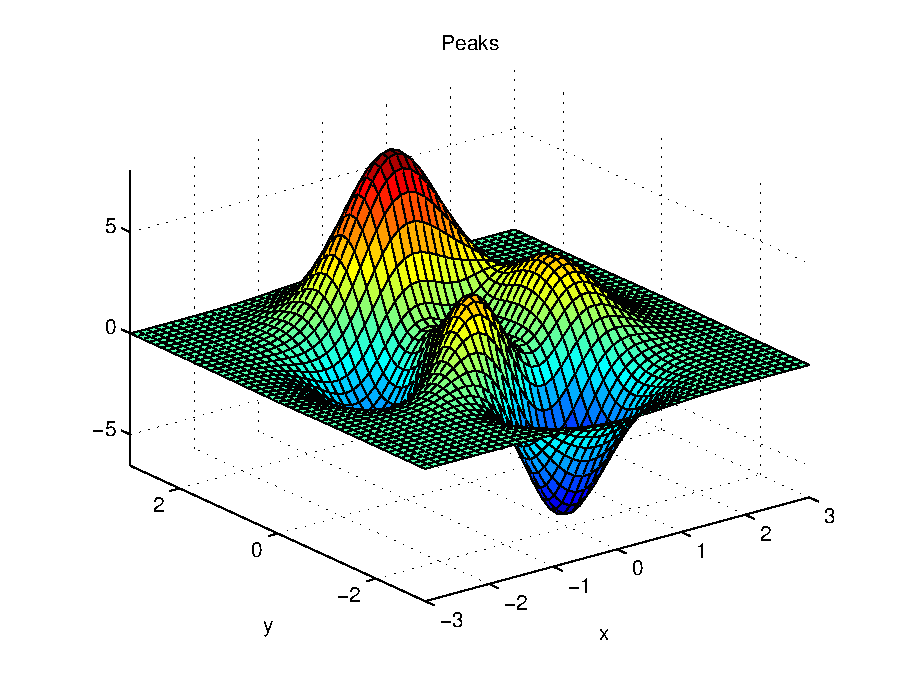
\includegraphics[width=12cm]{mcmthesis-aaa.eps}%Filename of figure here.
\caption{Figure name} \label{Label of figure}
\end{figure}

Here is an example to cite equation \eqref{aa}. Here is an example of equation with mark:
\begin{equation}
a^2 \label{aa}%Label of equation
\end{equation}

Here are some examples of equation without mark:
\[
  \begin{pmatrix}{*{20}c}
  {a_{11} } & {a_{12} } & {a_{13} }  \\
  {a_{21} } & {a_{22} } & {a_{23} }  \\
  {a_{31} } & {a_{32} } & {a_{33} }  \\
  \end{pmatrix}
  = \frac{{Opposite}}{{Hypotenuse}}\cos ^{ - 1} \theta \arcsin \theta
\]

\[
  p_{j}=\begin{cases} 0,&\text{if $j$ is odd}\\
  r!\,(-1)^{j/2},&\text{if $j$ is even}
  \end{cases}
\]
and equation marked manually:
\[
  \arcsin \theta  =
  \mathop{{\int\!\!\!\!\!\int\!\!\!\!\!\int}\mkern-31.2mu
  \bigodot}\limits_\varphi
  {\mathop {\lim }\limits_{x \to \infty } \frac{{n!}}{{r!\left( {n - r}
  \right)!}}} \eqno (1)
\]

\section{Terminologies and Notations}

\subsection{Terminologies}

\subsection{Notations}

Here is an example of table.
\begin{table}[h]
\centering
\caption{Caption of table}
\label{Label of table}
\begin{tabular}{c|lc}
\toprule
Symbols & Definitions & Unit\\
\midrule
x & Please write the definition of x here & Unit of x\\
Y & Definition of Y here & Unit of Y\\
\bottomrule
\end{tabular}
\end{table}

\section{Model One}

We assume that the environmental cost of a land use project is the reduction of ecosystem services due to the project. To quantify the equivalent economic value of services, we define, VES, the Value of  Ecosystem Services. Millennium Ecosystem Assessment classified the Ecosystem services into four categories: provisioning services, regulation services, cultural services and supporting service. Supporting services, the services that allow other ecosystem services to present, are included into other three kinds of ecosystem services in many context. Therefore, we divide VES into three components: value of provisioning services, value of regulation services and value of cultural services, which is showed in the equation below:
\begin{equation}
VES=v_{prov}+v_{reg}+v_{cul}
\end{equation}
where 

In next three subsections, we are going to determine influence variables of each component of VES and their relationship respectively.

\subsection{The cost of food product reduction}
In this subsection, we will investigate the function of value of provision services, $v_{prov}$. Provision services are defined as all the products obtained from the ecosystem. We choose three main kinds of products: air, water and agricultural/forestry product. 
\begin{equation}
v_{prov}=v{air}+v_{water}+v_{prod}
\end{equation}
where \begin{itemize}
\item $v_{prov}$ --- value of ecosystem's provisioning services
\item $v_{air}$ --- value of fresh air for breath provided by ecosystem
\item $v_{water}$ --- value of fresh drinking water provided by ecosystem
\item $v_{prod}$ --- value of agricultural products and forestry products provided by ecosystem
\end{itemize}

\noindent\textbf{Water Pollution}

The healthy growth of plants need water and air. Pollution of water and air tend to reduce the value of food and other organic materials (like wood) that ecosystem can provide us with. In this subsection, we look into cost caused by water pollution and air pollution.

The cost on $v_{prod}$ is mainly reflected in two aspect: the amount reduct and quality degradation of food. To get the former one, we times the reduced amount with the original market price of the agricultural product; as for the latter one, we times the reduced market price with the amount of agricultural influenced by polluted water. The reduced market price can difference of average price of healthy agricultural product and polluted agricultural product.
\begin{equation}
\Delta v_{prod,w}=\Sigma_{i=1}^{n}[a_{i1}P_iS_iQ_i+a_{i2}\beta_iP_iQ_i]
\end{equation}
where\begin{itemize}
\item $v_{prod,w}$ --- cost of agricultural product caused by water pollution
\item $a_{i1}$ --- reduced percentage of agricultural product $i$'s harvest amount due to water pollution
\item $a_{i2}$ --- reduced percentage of agricultural product $i$'s price due to water pollution
\item $S_i$ --- planting area of agricultural product $i$
\item $Q_i$ --- harvest amount of healthy agricultural product $i$
\end{itemize}
For simplicity, we choose several typical agricultural products to conduct the calculation. The species and  are showed in the following table.

\subsection{Local Assumption}

\subsection{Model Establishment}

\subsection{Model Result}

\section{Extended Model}

\section{Sensitivity Analysis}

\section{Conclusions}

\section{Strengths and weaknesses}

\subsection{Strengths}
\begin{itemize}
\item \textbf{Applies widely}\\
This  system can be used for many types of airplanes, and it also
solves the interference during  the procedure of the boarding
airplane,as described above we can get to the  optimization
boarding time.We also know that all the service is automate.
\item \textbf{Improve the quality of the airport service}\\
Balancing the cost of the cost and the benefit, it will bring in
more convenient  for airport and passengers.It also saves many
human resources for the airline.
\end{itemize}

\subsection{Weakness}

\addcontentsline{toc}{section}{Reference}
\bibliography{1901923.bib}
\bibliographystyle{siam}%unsrt按引用先后排序

\begin{appendices}

\section{First appendix}

Here is example of inserting code. Here are simulation programs we used in our model as follow.\\

\textbf{\textcolor[rgb]{0.98,0.00,0.00}{Input matlab source:}}
\lstinputlisting[language=Matlab]{./code/mcmthesis-matlab1.m}%Matlab code path

\section{Second appendix}

some more text \textcolor[rgb]{0.98,0.00,0.00}{\textbf{Input C++ source:}}
\lstinputlisting[language=C++]{./code/mcmthesis-sudoku.cpp}

\end{appendices}
\end{document}
